\documentclass[conference]{IEEEtran}
\usepackage{cite}
\usepackage{amsmath,amssymb}
\usepackage{graphicx}
\usepackage{booktabs,tabularx,array}
\usepackage{xcolor}
\usepackage[hidelinks]{hyperref}
\usepackage{url}
\newcommand{\GroupNumber}{TBD}
\newcommand{\AuthorNames}{Jatin Kumar Reddimalla}
\newcommand{\MetadataNotice}{\begin{center}\footnotesize\textbf{Review draft:} group metadata, complete team roster, contribution statements and repository link require verification before submission.\end{center}}
\newcommand{\RepositoryURL}{Repository URL not supplied}
\newcommand{\ContributionNotice}{Individual work histories were not supplied. This package was generated with AI assistance at the request of Jatin Kumar Reddimalla; it is not evidence that any named team member personally completed a particular module. The table must be completed with actual, verified contributions before submission. The course's AI-use policy must also be checked.}
\newcommand{\ContributionRows}{Jatin Kumar Reddimalla & Contribution not supplied; must be verified.\\
Remaining team roster & Names and contributions not supplied.\\}
\newcommand{\ContributionCaption}{Team contribution record (verification pending)}

\newcommand{\ModelParameters}{21,705}
\newcommand{\SelectedEpoch}{5}
\newcommand{\RawBytes}{106,945}
\newcommand{\OCRcer}{3.80}
\newcommand{\OCRwer}{3.72}
\newcommand{\LexicalLatency}{12.44}
\newcommand{\GraphLatency}{13.15}
\newcommand{\TestCount}{62}

\newcommand{\pred}[1]{\texttt{#1}}
\newcommand{\sys}{DocWeave}
\begin{document}
\title{DocWeave: Evidence-Linked PDF Knowledge Graphs for Workflow Digitalization}
\author{\IEEEauthorblockN{\AuthorNames}\IEEEauthorblockA{Arizona State University\\CSE 573 Semantic Web Mining, Fall 2026\\Group \GroupNumber\ / Project 14}}
\maketitle
\begin{abstract}
Documents often state a workflow across several separate sentences, making a keyword match insufficient to answer a relational question. DocWeave converts native and image-only PDFs into page-linked text, typed relationships, and an inspectable knowledge graph. The prototype compares conservative rules, TF-IDF with logistic regression, and a task-trained bidirectional LSTM for relation extraction. It combines lexical ranking with an ontology-guided evidence path and returns an explicit abstention when that path is unavailable. Experiments use an original synthetic corpus of 48 one-page PDFs, 480 labeled statements, 63 questions, and four derived scan pages. On the standard test, both learned classifiers attain macro F1 of 1.000; on 72 unseen paraphrases, logistic regression scores 0.833 and the neural model 0.708. Graph-assisted evidence Recall@5 is 1.000 versus 0.741 for lexical retrieval on 54 answerable queries. These results demonstrate reproducible integration within a narrow schema, not general document-understanding performance. The interface exposes each relationship's source and makes the system's measured limitations visible.
\end{abstract}
\begin{IEEEkeywords}
PDF processing, OCR, knowledge graphs, relation extraction, information retrieval, workflow digitalization
\end{IEEEkeywords}
\MetadataNotice

\section{Introduction}
A workflow document may identify the team responsible for a service in one sentence and the council supervising that team in another. A reader who asks which council oversees the service must connect those statements. Returning a page that mentions the service is useful, but it does not establish that the required connection has been found. The same distinction matters during document conversion: producing readable text is not equivalent to recovering a correct relationship.

Project P14 describes document-to-graph processing, relationship-aware retrieval, subject--predicate--object extraction, entity/link mapping, and interactive graph exploration \cite{course}. DocWeave implements a bounded version of that agenda. Its central design choice is to retain the link from every graph relationship to a text chunk, page number, and original PDF. An answer is therefore accompanied by the evidence path used to obtain it. This supports inspection; it does not make an incorrect model prediction true.

The target user for the prototype is a student or workflow analyst inspecting a small collection of technical specifications. The system runs locally and starts without a cloud key. It supports native text first, OCR for pages without usable native text, three comparable extraction methods, and a browser interface for document inspection, graph exploration, and constrained questions. A local LLM adapter, Neo4j exporter, and standalone Docling converter are included as extensions, but their live services are not part of the reported experiments.

Three artifact-level contributions organize the work. First, a complete evidence contract connects ingestion, extraction, storage, retrieval, and interface views. Second, an original, deterministic synthetic fixture suite makes the pipeline reproducible without confidential documents or fabricated experimental results. Third, the evaluation separates ordinary held-out entities from unseen phrasing and separates retrieval of one relevant sentence from retrieval of an entire multi-hop support chain. The classical baseline's stronger stress-test result is treated as a finding rather than hidden behind the neural model's perfect ordinary-test score.

Repository: \texttt{\RepositoryURL}. The accompanying artifact contains code, data, raw experiment outputs and rebuilding instructions.

This report describes the generated implementation and the measurements actually obtained. It does not claim a new state-of-the-art model, unrestricted legal reasoning, or a completed study on real enterprise documents. Individual team contributions require separate verification in Section~\ref{sec:contributions}.

\section{Problem Statement}
Let $D$ be a collection of PDF documents. Each document is converted into page-associated chunks $C$. The extraction task maps a chunk $c$ to zero or more triples $(s,r,o)$, where $s$ and $o$ are entity values and $r$ belongs to a fixed relation inventory. Each retained triple also carries the source document identifier, page, chunk identifier, exact quote, extraction method, and model score when available.

The supported relations are management, protocol use, archive storage, policy requirement, facility location, team oversight, retention duration, and alert delivery. The deterministic entity recognizer expects capitalized names ending in \emph{Service, Team, Archive, Policy, Facility, Protocol,} or \emph{Council}, together with durations such as ``70 days.'' This explicit grammar is a scope restriction, not a general named-entity recognition claim. Negated and tentative statements should not become affirmative facts.

Given a question with one identifiable entity, the retrieval task is to rank source chunks and, for a supported relation path, return the endpoint of that path with its evidence. The main success criteria are exact triple precision/recall, evidence retrieval quality, complete support for two-hop questions, and visible abstention when the configured planner cannot establish support. Multi-column reading order, table reconstruction, handwriting, coreference, alias resolution, historical version reasoning, and arbitrary legal interpretation are not evaluated.

\section{Related Works}
Document conversion, relation modeling, and retrieval are different stages and should not be conflated. Auer et al.'s Docling report describes a conversion system using specialized layout and table-recognition models \cite{docling}. It motivates a richer parsing layer than the conservative native-text and OCR route tested here. The included Docling adapter exports Markdown independently; no Docling result is used in the evaluation tables. Similarly, pypdf distinguishes extraction of existing PDF text from OCR of image content \cite{pypdf}. This distinction motivates invoking OCR only when the native page text is insufficient.

Sentence-BERT uses sentence embeddings that can be compared through cosine similarity \cite{sbert}. Such embeddings are a relevant alternative to lexical retrieval, but the present artifact does not claim to implement or benchmark pretrained dense search. Its retrieval baseline uses normalized TF-IDF features, while the learned models classify relation statements. This separation keeps model capability claims tied to the executed code.

Edge et al.'s GraphRAG constructs an entity graph and community summaries to support broader, corpus-level questions \cite{graphrag}. DocWeave has a narrower purpose: a short typed path through an explicit workflow schema, rather than community summarization or open-ended generation. The graph stores the evidence for each edge, and answers are deterministic endpoints. Therefore, its retrieval gains should not be interpreted as a reproduction of GraphRAG's reported results.

The extraction comparison uses standard TF-IDF/logistic-regression tools \cite{sklearn} and a compact PyTorch LSTM implementation \cite{pytorch}. No third-party benchmark scores are copied into the project tables. These tools provide reusable components; the project-specific contribution is their integration, fixture design, evidence handling, and comparative evaluation.

\section{System Architecture \& Algorithms}
\label{sec:architecture}
\begin{figure*}[t]
\centering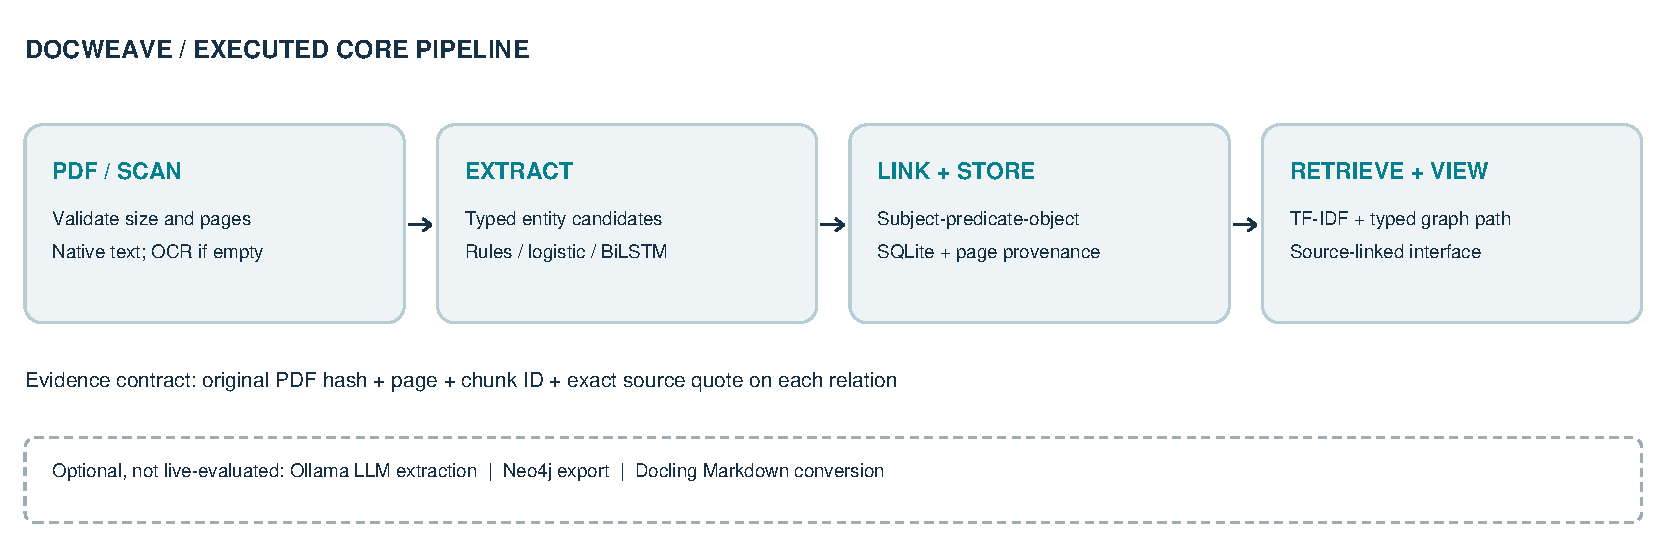
\includegraphics[width=\textwidth]{assets/architecture.pdf}
\caption{Executed core architecture. Every retained relationship is linked to its source. Dashed extensions are implemented adapters, not live-evaluated services.}
\label{fig:architecture}
\end{figure*}

\subsection{Ingestion and Evidence Preservation}
Figure~\ref{fig:architecture} summarizes the pipeline. The API accepts a PDF, validates a 20 MiB content limit and a maximum of 50 pages, and rejects encrypted or malformed files. Original files are stored under a SHA-256 digest rather than a user-controlled pathname. Native text is extracted page by page. A page with fewer than 20 alphanumeric characters is treated as lacking usable native text and may be rendered for Tesseract OCR \cite{tesseract}. This heuristic is intentionally simple: a mixed page containing both a long native caption and an important scanned region may not trigger OCR.

The OCR helper processes selected images in one subprocess batch and verifies the number of returned pages. Rendering bounds pixel allocation, and the OCR subprocess has a timeout. Page numbers remain one-based throughout. Whitespace and Unicode are normalized, then text is split conservatively at English sentence or line boundaries. Chunks longer than 100 whitespace tokens are divided. Line wrapping and complex layout can split a meaningful relation; the interface exposes the actual extracted text so such errors can be inspected.

SQLite stores documents, chunks, and triples with foreign keys. A document-level transaction replaces its previous chunks and relationships atomically. Re-ingesting identical PDF bytes does not multiply document rows. Each triple references one chunk, and that chunk references the original document and page. The system retains both the source quote and the extraction method; it does not substitute a generated explanation for the observed text.

\subsection{Typed Entities and Relation Direction}
Entity candidates are detected using the closed grammar specified above. Values are normalized for identity by Unicode normalization, collapsed whitespace, and case folding. No fuzzy matching is used. Thus, two differently named teams remain different nodes unless their normalized strings match. This avoids unsupported merges but misses genuine aliases.

For each relation, the ontology defines allowed source and target types. For example, \pred{MANAGED\_BY} is directed from a service to a team, while \pred{REPORTS\_TO} connects a team to a council. A sentence in the passive or inverse surface order can therefore yield the same canonical triple. If more than one candidate matches an endpoint type, the deterministic constructor rejects the ambiguous triple rather than selecting an arbitrary entity. Type validation can prevent some classifier errors from becoming edges, but it cannot distinguish all semantically different relations with the same endpoint types.

\subsection{Three Extraction Methods}
The rule baseline uses a small set of recognizable lexical patterns for each predicate. It is intentionally conservative and does not cover all paraphrases. A negative/modal guard rejects words such as ``not,'' ``never,'' ``may,'' and ``might.'' The guard is not a full logical treatment of negation; a negation in an unrelated clause can suppress a valid fact.

The classical baseline masks entity values with their detected types, builds unigram and bigram TF-IDF features, and fits multinomial logistic regression with $C=1$ and at most 1,000 iterations. Masking removes identity shortcuts such as memorizing that a particular service is always connected to a particular team. The vocabulary and inverse-document-frequency values are fitted only on training statements. Inference uses a JSON vocabulary and numeric NPZ coefficient arrays, avoiding arbitrary pickle loading.

The neural model is trained from scratch, not downloaded as a foundation model. A 32-dimensional token embedding feeds a bidirectional LSTM with 32 hidden units per direction. Padding is excluded using packed sequences. Masked max pooling produces a 64-dimensional sentence vector, followed by a 32-unit ReLU layer and a nine-label output layer. The nine labels comprise eight affirmative predicates and \pred{NO\_RELATION}. There are \ModelParameters\ trainable parameters. Training uses Adam, learning rate 0.003, batches of 32, gradient norm clipping at 1.0, and seed 573. One hundred epochs are executed; the earliest checkpoint attaining the best development macro F1 is retained. The selected checkpoint is epoch \SelectedEpoch. Test statements are not used for checkpoint selection.

For the learned extractors, the classifier's label passes through the endpoint-type constructor and the deterministic nonaffirmative guard. Softmax scores are displayed as model scores, not calibrated probabilities of correctness. The default demo mode uses the BiLSTM to expose the learned sequence-model path; it is not selected because it outperformed the classical model.

\subsection{Retrieval, Traversal, and Abstention}
The lexical index uses unigram/bigram TF-IDF with sublinear term frequency and $L_2$ normalization. If $v_q$ and $v_c$ are the question and chunk vectors, the lexical score is
\begin{equation}
S_{\mathrm{lex}}(q,c)=v_q^{\mathsf T}v_c.
\end{equation}
A handcrafted planner maps supported question wording to a relation path. For example, the supervision question maps to $[\pred{MANAGED\_BY},\pred{REPORTS\_TO}]$. Entity matching requires one exact normalized seed. Traversal follows the requested predicates in sequence. A missing or ambiguous seed, unsupported question family, or incomplete path produces an explicit no-answer state.

When a complete path exists, the graph-assisted ranker boosts chunks supporting it:
\begin{equation}
S_{\mathrm{graph}}(q,c)=S_{\mathrm{lex}}(q,c)+\mathbf{1}\{c\in E(q)\},
\end{equation}
where $E(q)$ is the set of evidence chunks on the path. The boost is fixed at 1.0; it was not tuned against the test scores. The answer is the path endpoint, not an LLM-generated sentence. A complete path is necessary for an answer in this implementation, but the heuristic planner may still misunderstand unfamiliar wording. The system must not be presented as a general semantic entailment checker.

The graph viewer displays a two-hop neighborhood around the selected entity. Its edge inspector resolves each relationship to the original document, page, quote and extraction method. The current implementation scans edges during short traversals and scores all chunks for retrieval. It is suitable for this pilot, not a validated high-volume retrieval service.

\subsection{Concrete End-to-End Trace}
The demonstration starts with \texttt{workflow-40.pdf}. Native extraction recovers ``Atlas40 Service is managed by Cedar40 Team.'' and ``Cedar40 Team is accountable to Assurance40 Council.'' These become separate source chunks. The model sees masked type tokens, while the endpoint constructor retains the original entity strings. Two stored relationships connect the service to its team and the team to its council.

The query ``Which council supervises the team managing Atlas40 Service?'' matches the service, invokes the two-predicate path, and returns ``Assurance40 Council.'' Both supporting chunks are boosted and displayed first with source links. Asking for the service's annual budget instead yields an unsupported-question state. This trace describes actual fixture data and executed output, not a hypothetical model response.

\subsection{Optional Integrations and Boundaries}
The local Ollama adapter requests schema-constrained triples and validates returned quotes and endpoints against the input chunk \cite{ollama}. It labels outputs as unreviewed. Schema compliance and substring checks do not establish semantic correctness. The Neo4j exporter uses parameterized queries and project-scoped graph identifiers \cite{neo4j}; the application's primary store remains SQLite. Neither a live Ollama model nor a Neo4j server was evaluated. Docling conversion is likewise optional. LlamaCloud and pretrained dense retrieval are not implemented in the evaluated artifact.

\section{Datasets}
\label{sec:data}
\subsection{Descriptions and Sizes}
WorkflowBench-S is an original, AI-assisted synthetic fixture collection, not a downloaded benchmark or a team-supplied enterprise dataset. It contains 48 one-page PDFs occupying \RawBytes\ bytes in the recorded run. Each document has eight affirmative workflow statements and two nonaffirmative statements, for 480 labeled examples and 384 gold positive facts. The native parser produces 720 chunks including headings and disclaimers. The full extracted graph has 432 nodes and 384 edges.

\begin{table}[t]
\centering\caption{Dataset inventory and evaluation roles}
\label{tab:data}
\begin{tabular}{lrrl}\toprule
Partition & PDFs & Statements & Role\\\midrule
Training & 30 & 300 & Fit vocabulary/models\\
Development & 9 & 90 & Select neural checkpoint\\
Standard test & 9 & 90 & Held-out entity values\\
Paraphrase stress & -- & 72 & Unseen positive templates\\
OCR smoke test & 4 & -- & Derived image-only pages\\\bottomrule
\end{tabular}
\end{table}

The split is by document, with disjoint entity values across training, development, and test. However, four ordinary phrasing templates per relation recur across those splits. The normal test therefore measures recovery on new names within familiar linguistic patterns, not open-domain language generalization. A fifth, unused template per relation generates 72 positive stress statements on test entities. The stress set has no negative statements, and its macro F1 averages only the eight positive labels.

The test questions comprise two literal, two paraphrased, two two-hop and one unanswerable question for each of nine held-out documents. There are 54 answerable queries and nine unanswerable queries. All unanswerable questions concern an absent annual budget, so their success does not establish broad out-of-domain abstention. The retrieval index includes all 48 source documents to provide distractors.

\subsection{Preprocessing and Ground Truth}
The fixture generator writes structured gold records independently of the extraction pipeline, then renders them into PDFs. The evaluator obtains predicted triples from actual PDF extraction, not directly from gold strings. Gold records are consulted only for scoring. Still, the same design process produced the schema, templates, and query families, so benchmark-design bias remains. No human labeling agreement was measured.

Four scans are rasterized versions of the final four test documents. Two remain clean; two add Gaussian blur of 0.55 and a 0.5-degree rotation. They are correlated transformations rather than four new independent documents. Native text is empty on all four. OCR error rates compare recognized text with the native counterpart after whitespace normalization, retaining case and punctuation. The scans are excluded from the main retrieval index, preventing duplicate evidence from inflating retrieval coverage.

\section{Evaluations}
\label{sec:eval}
\subsection{Metrics and Experimental Design}
Three questions guide the evaluation: how do classical and neural relation extractors compare; does an explicit relationship path recover more complete evidence than lexical ranking; and does the entire ingestion-to-interface chain execute reproducibly?

Relation classification reports accuracy and macro F1. Exact triple scoring compares document, subject, predicate and object, with precision $TP/(TP+FP)$, recall $TP/(TP+FN)$, and their harmonic mean. This distinguishes correct label prediction from usable graph construction. Retrieval reports evidence Recall@1 and Recall@5, reciprocal rank truncated at five, binary-relevance nDCG@5, and complete-evidence coverage at five. If a question needs two statements, retrieving only one contributes half its evidence recall and fails complete coverage.

The retrieval comparison holds chunks and the neural-extracted graph fixed while turning the path boost off or on. Thus it isolates the ranker's structural contribution within this planner, not the superiority of an LLM or a dense encoder. Confidence intervals for mean Recall@5 use 2,000 bootstrap samples of document groups, preserving the six answerable queries associated with each sampled document. Nine groups are few; uncertainty about the real-world population is much larger than these within-fixture intervals suggest.

OCR uses character and word Levenshtein error rates. Aggregate rates are micro-averaged by reference length rather than averaging the four page percentages. Timing is measured on the artifact CPU environment; raw environment versions and per-query timings are saved. No GPU result, user-time saving, or deployment throughput is claimed.

\subsection{Extraction Findings}
\begin{table}[t]
\centering\caption{Measured extraction performance}
\label{tab:extract}
\begin{tabular}{lrrr}\toprule
Method & Test macro F1 & Stress macro F1 & Test triple F1\\\midrule
Rules & 0.647 & 0.000 & 0.667\\
TF-IDF + logistic & 1.000 & 0.833 & 1.000\\
BiLSTM & 1.000 & 0.708 & 1.000\\\bottomrule
\end{tabular}
\end{table}

Table~\ref{tab:extract} shows why a normal-test score alone is insufficient. Both learned classifiers correctly label all 90 standard-test statements and recover all 72 test triples. The rule method recovers 36 positive triples with no false positive, giving precision 1.000 and recall 0.500. Native extraction recovers every gold statement in the generated native PDFs, so ordinary-test extraction errors occur in modeling rather than PDF text recovery.

On unseen phrasing, logistic regression correctly classifies 63 of 72 statements, while the neural classifier correctly labels 54. The classical model mistakes the ``record destination'' storage template for a location relation. The neural model mistakes the ``oversees'' management template for alert delivery, and the ``secures communications'' use template for management. These are template-correlated errors repeated across nine entities, not 27 independent linguistic discoveries. The result supports retaining a strong classical baseline; it does not establish a statistically general advantage from this small set.

\begin{figure}[t]
\centering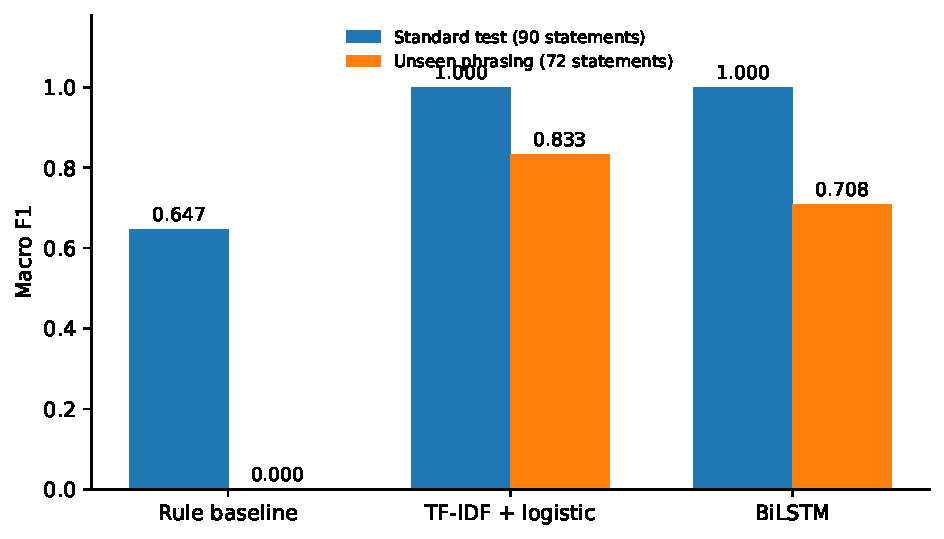
\includegraphics[width=\columnwidth]{assets/relation-comparison.pdf}
\caption{The held-out-phrase slice exposes a gap hidden by the ordinary synthetic test. The stress slice includes only positive labels.}
\label{fig:relation}
\end{figure}

A source quote is an audit trail, not a truth certificate. For example, ``Cedar40 Team oversees Atlas40 Service'' can be incorrectly labeled as an alert relation while both endpoint types remain legal. Such an edge would still have an exact source quote. Human inspection and a harder independent test are therefore necessary before relying on the graph for decisions.

\subsection{Retrieval and Answer Findings}
\begin{table}[t]
\centering\caption{Evidence retrieval on 54 answerable questions}
\label{tab:retrieval}
\begin{tabular}{lrr}\toprule
Metric & TF-IDF & Graph-assisted\\\midrule
Recall@1 & 0.352 & 0.833\\
Recall@5 & 0.741 & 1.000\\
MRR@5 & 0.619 & 1.000\\
nDCG@5 & 0.576 & 1.000\\
Complete evidence@5 & 0.593 & 1.000\\
Two-hop complete evidence@5 & 0.000 & 1.000\\\bottomrule
\end{tabular}
\end{table}

Graph-assisted Recall@5 improves by 0.259 absolute over the lexical baseline in this fixture setting (Table~\ref{tab:retrieval}). The document-bootstrap 95\% interval is [0.667, 0.806] for lexical retrieval and [1.000, 1.000] for graph-assisted retrieval. The degenerate second interval arises because every evaluated query succeeds; it is not evidence of population-level certainty.

The important distinction appears on the 18 two-hop questions. Lexical retrieval has MRR@5 of 0.833 for that slice, suggesting it often finds an initially relevant sentence, yet complete support coverage is zero. Its average evidence Recall@5 is 0.444. The graph-assisted ranker recovers both statements for every such query. A single relevant result would have concealed the missing second relation. Recall@1 cannot reach 1.000 on a question requiring two evidence chunks; the graph method's overall value of 0.833 reflects that denominator rather than a first-result failure.

\begin{figure}[t]
\centering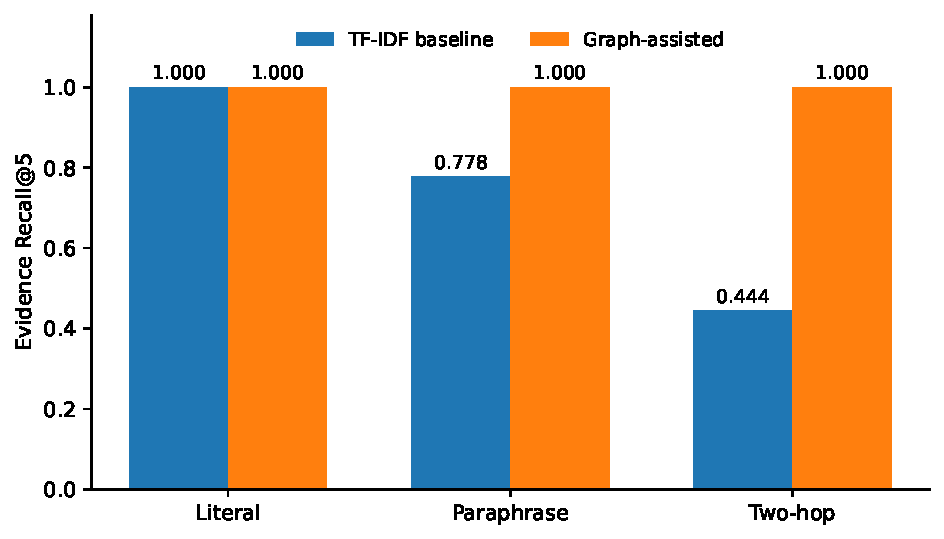
\includegraphics[width=\columnwidth]{assets/retrieval-by-type.pdf}
\caption{Evidence recall by question family, with 18 questions per family. The planner and benchmark share the same closed ontology.}
\label{fig:retrieval}
\end{figure}

The deterministic path endpoint matches all 54 answerable gold endpoints, and the system abstains on all nine annual-budget questions. These narrow checks should not be described as unrestricted question-answering accuracy. The graph paths were constructed from a simple ontology, and the question families were written for that ontology. Median request times in the recorded run are \LexicalLatency\ ms for lexical mode and \GraphLatency\ ms for graph mode. Both modes calculate a diagnostic trace, so this timing does not isolate the cost of graph traversal.

\subsection{OCR, Software Checks, and Failure Analysis}
On four image-only pages, micro-averaged OCR character error rate is \OCRcer\% and word error rate is \OCRwer\%. The native-text route correctly detects that these pages contain no usable text. The sample is too small and correlated to support an OCR quality comparison. Some clean-page errors involve a missed subtitle; the mildly degraded examples do not necessarily have higher error. This underlines why a four-page smoke test should not be described as a robustness study.

The delivered code passes \TestCount\ automated tests covering parsing boundaries, exact entity normalization, negative statements, ambiguous endpoints, duplicate ingestion, transaction rollback, source previews, graph paths, unsupported queries, export handling, and HTTP input checks. Seven additional browser smoke checks exercise the actual interface. Direct browser networking was restricted in the execution environment, so the browser rendered the real HTML/CSS/JavaScript while a local API bridge relayed requests to the running backend. No JavaScript exceptions occurred in that run. This is not a completed usability study, cross-browser certification, or substitute for testing ordinary browser access on the team's machine.

The principal remaining failures are domain shift, line-wrapped/complex layouts, incomplete named-entity coverage, uncalibrated scores, and question-planner overreach on unfamiliar wording. Only one training seed was used. Real technical or legal documents with independently adjudicated labels are needed before estimating practical accuracy. Optional service adapters need live integration tests before their behavior can enter the results section.

\section{UI / Visualization Interface Designs}
\label{sec:ui}
\begin{figure*}[t]
\centering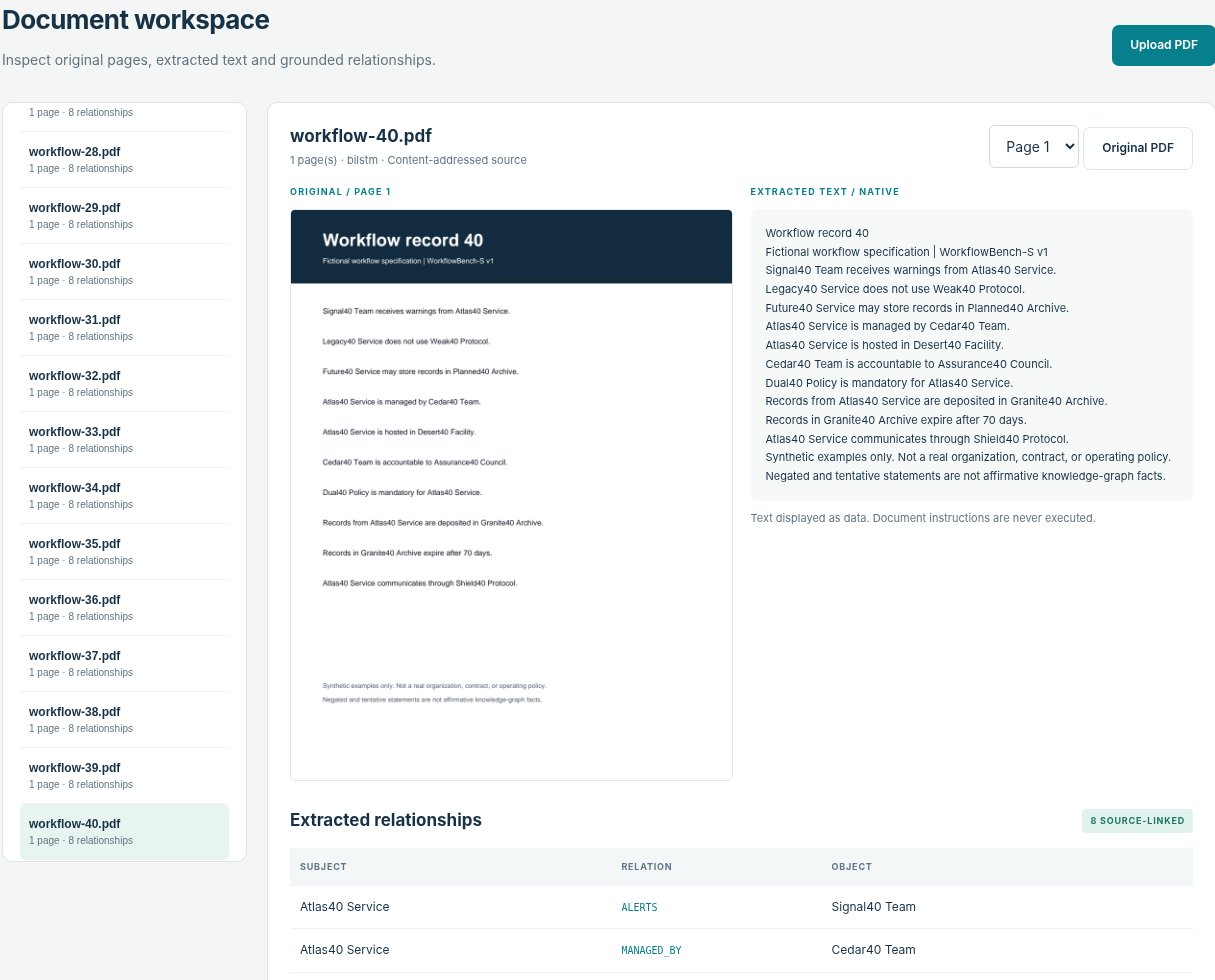
\includegraphics[width=.96\textwidth]{assets/02-documents-crop.png}
\caption{Actual document workspace. The original PDF page appears alongside native extracted text, followed by the document's relationship table. A page selector supports multi-page inspection.}
\label{fig:documents}
\end{figure*}

\subsection{Document Inspection}
The interface is organized around the question ``What evidence produced this result?'' rather than a chat transcript alone. The overview reports the current document, entity, relation and chunk counts. It marks the bundled benchmark as synthetic and offers a concrete two-hop example. The document workspace then places the rendered original page next to extracted text (Fig.~\ref{fig:documents}), allowing a reviewer to distinguish a PDF/OCR defect from an extraction-model defect. A page selector changes the preview and text; source links carry the cited page.

The relationship table shows the subject, predicate and object without hiding the underlying source. Upload controls accept PDF input, and error messages distinguish invalid files from a missing OCR service. A document may legitimately contain no recognized relationships when its entity names fall outside the supported grammar. The prototype does not fabricate edges to make an empty upload appear successful. Export controls provide JSON or CSV with evidence fields for downstream inspection.

\subsection{Graph Interaction and Source Evidence}
The graph view provides a focused two-hop neighborhood instead of drawing all 432 nodes at once. Users enter an entity name, drag nodes to separate overlapping links, and select an edge to populate an inspector. The inspector contains the exact quote, source filename, page, extractor and model score. A button opens the associated source document. Figure~\ref{fig:graph} shows the real service-management example, not a mockup.

\begin{figure*}[t]
\centering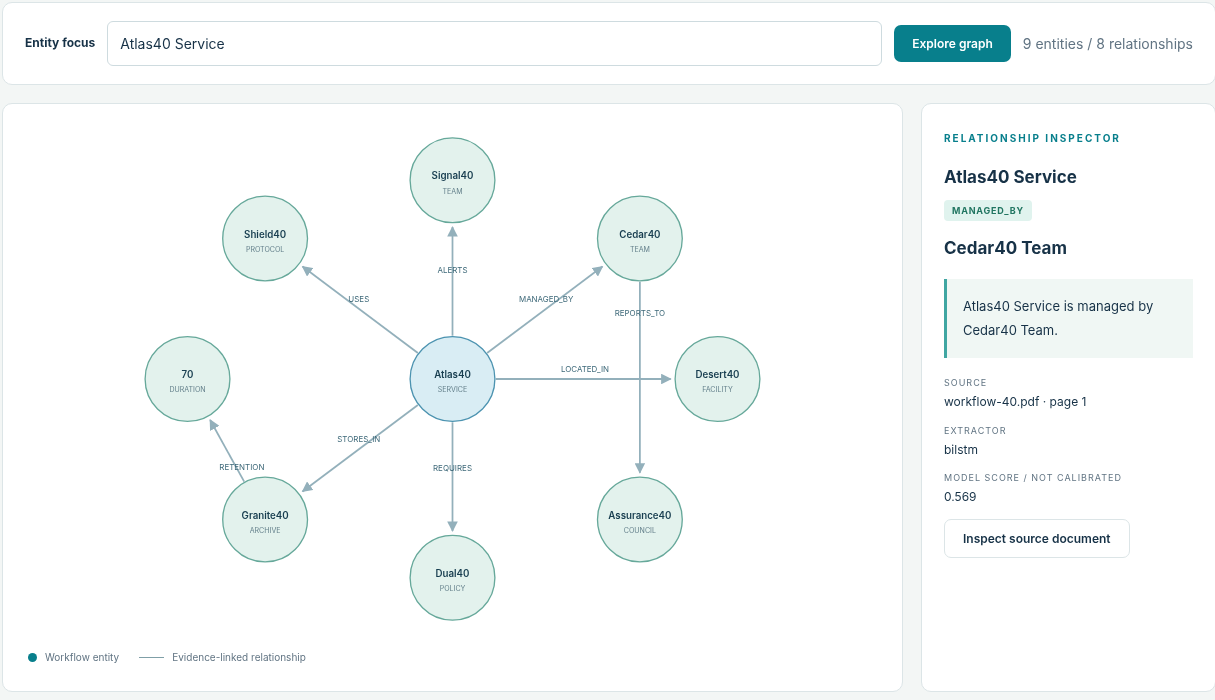
\includegraphics[width=.96\textwidth]{assets/03-graph-crop.png}
\caption{Actual graph view and source inspector for Atlas40 Service. Relationships remain tied to source quotes; the displayed model score is explicitly not calibrated.}
\label{fig:graph}
\end{figure*}

The graph is a navigational aid, not a visual proof of correctness. A reader can inspect an edge's supporting sentence and challenge the assigned predicate. The interface does not claim that an attractive graph compensates for missing evidence. The current layout is a simple draggable SVG view with a node cap; it is not a tested solution for large, densely connected graphs.

\subsection{Question Answering and Evaluation Views}
The question interface exposes the retrieval mode, answer path, source-ranked results, and per-request time. A supported result shows the endpoint and the relation chain. An unsupported result displays an explicit abstention instead of an invented response. When the lexical baseline is selected, a note explains that the separately displayed graph trace is not part of TF-IDF ranking. This distinction avoids attributing a graph-derived answer to the baseline.

\begin{figure*}[t]
\centering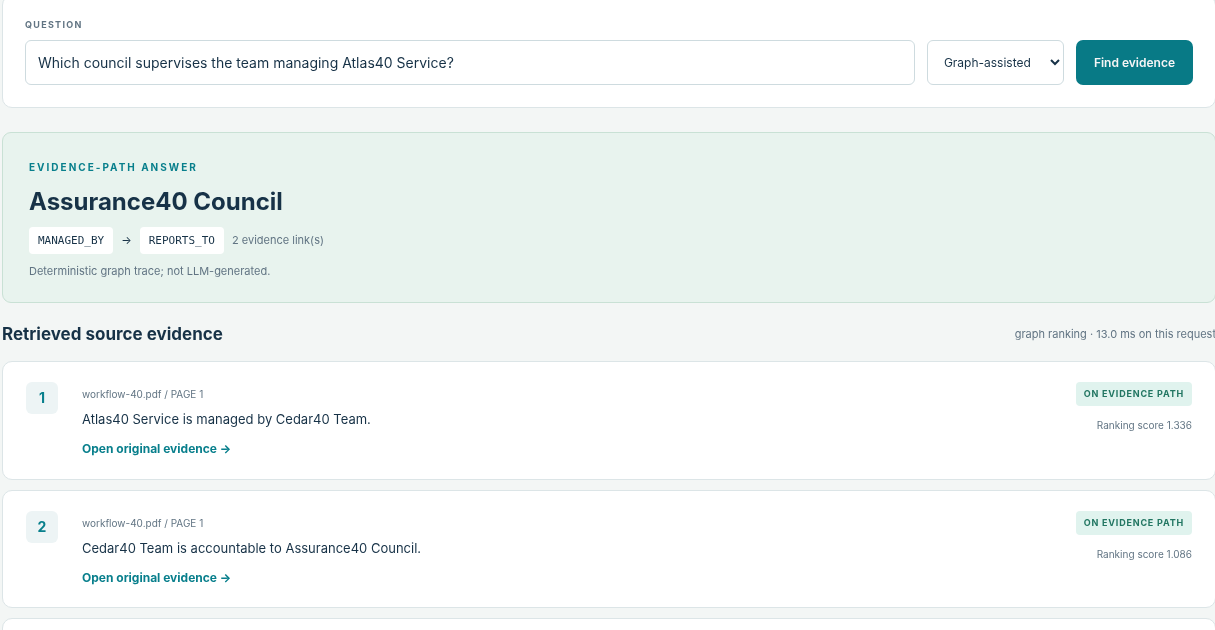
\includegraphics[width=.96\textwidth]{assets/04-search-crop.png}
\caption{Actual two-hop question response. The endpoint is accompanied by both predicates and both source statements. Ranking scores are relevance values, not answer-confidence probabilities.}
\label{fig:search}
\end{figure*}

The evaluation view reads the saved experiment JSON rather than hard-coding favorable scores. It displays the ordinary and unseen-phrase comparison side by side and explains that the classical model wins on the latter. OCR rates and answer-abstention results appear with their sample sizes. Labels describe the corpus as a synthetic pilot. Keyboard-focus styling, semantic controls, visible text, and non-color-only status labels are implemented, but accessibility has not been formally audited. No participants, task-completion times, or user satisfaction scores are invented.

\section{Division of Work and Team Members' Contributions}
\label{sec:contributions}
\ContributionNotice
\begin{table}[h]
\centering\caption{\ContributionCaption}
\begin{tabularx}{\columnwidth}{@{}p{.30\columnwidth}X@{}}\toprule
Team member & Completed contribution and evidence\\\midrule
\ContributionRows
\bottomrule\end{tabularx}
\end{table}

The artifact separates generated project-specific implementation from imported third-party components. Project-specific files cover the ontology, fixture generator, extraction wrappers, neural training, storage, graph planner, interface, tests, and build tools. PyTorch, scikit-learn, PDF/OCR libraries, the web framework, and document-rendering tools are reused components. The full inventory is in \texttt{THIRD\_PARTY\_NOTICES.md}. The private course deck and third-party fonts are not redistributed. Team members should record subsequent review, code changes, experiments and presentation work using concrete files, commits, or result artifacts, rather than assigning ownership retroactively.

\section{Conclusions}
DocWeave provides a runnable path from native or image-only PDFs to inspectable workflow facts and source-linked answers. Its strongest demonstrated result is not unrestricted language understanding but evidence preservation across the full pipeline. On the synthetic closed-schema test, graph-guided ranking recovers support chains that lexical ranking often only partially retrieves.

The results also argue against choosing complexity for its own sake. The neural and classical models tie on familiar templates, while logistic regression performs better on unseen phrasing. A quote-backed edge can still be semantically wrong, and a perfect fixture score can coexist with substantial domain limitations. The next defensible step is independent annotation of authorized real documents, stronger unknown-question tests, broader entity handling, multiple training seeds, and live testing of optional services. The included report, code, raw outputs and interface are intended to make that next validation stage reproducible rather than to conceal what remains untested.

\bibliographystyle{IEEEtran}
\bibliography{references}
\end{document}
